% \chapter{Theoretical Backgound}
\chapter{Fundamente teoretice}
\label{cap:fund-teoretice}


 În acest capitol sunt evidențiate și explicate pe scurt aspectele teoretice pe care se bazează proiectul. 

%
%Aici se descriu pe scurt aspecte teoretice pe care se bazează lucrarea. Conținutul acestui capitol trebuie gândit pentru un citor care nu e specializat pe domeniul temei și nu cunoaște chestiunile de bază despre subiect. Pentru un cititor specializat, capitolul poate să stabilească un limbaj comun, relativ la termenii care pot fi interpretați diferit. 
%
%Acest capitol nu trebuie gândit și scris nici ca un copy-paste din alte surse, nici ca zona de reglaj a numărului de pagini ale lucrării. Deși va conține chestiuni pe care le-ați studiat și voi și pe care v-ați bazat, el trebuie să fie o compilare a surselor folosite, care să aibă sens și relevanță pentru lucrarea voastră. Trebuie să fie o descriere coerentă și logică a unor aspecte care ușurează sau fac posibilă înțelegerea părților următoare ale lucrării. Nu trebuie intrat insă prea mult în detalii, ci spuse doar chestiunile esențiale. 
%
%Dacă preluați text, figuri, tabela etc. din sursele de documentare, acestea din urmă trebuie indicate explicit. 
%
%Reprezintă cca. 10--15\% din lucrare.
\section{Reverse proxy}

Un reverse proxy este un server intermediar care trimite mai departe request-urile pentru conținut, de la mai mulți clienți nedefiniți, către unul sau mai multe servere. Un reverse proxy este un tip de proxy care în mod normal este situat în spatele unui firewall într-o rețea internă și redirecționează traficul clienților către serverele asociate. Acesta introduce un nivel în plus de abstractizare și control, asigurând controlul fluxului de trafic  \cite{rev_proxy_server}.

\begin{figure}[h]
	\centering
	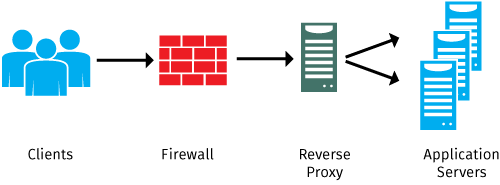
\includegraphics[width=0.6\textwidth]{rev-proxy.png}
	\caption{ Folosirea unui reverse proxy în arhitectura unei aplicații.}
	\label{fig:rev-proxy}
\end{figure}

Figura ~\ref{fig:rev-proxy} prezintă modalitatea de integrare a unui reverse proxy în implementarea arhitecturii de back end a unei aplicații. \\

Cele mai obișnuite caracteristici ce pot fi oferite de utilizarea unui reverse proxy sunt: 
\begin{itemize}
	\item Load balancing-un reverse proxy poate să distribuie request-urile primite de la clienți, astfel încât nici un server să nu fie copleșit ce reqesturi. În cazul în care un server este supraîncărcat cu reqest-uri sau este căzut, acesta poate să redirecționeze traficul carea alte servere funcționale. 
	\item Web acceleration - un reverse proxy poate să realizeze compresia datelor sau să memoreze în memoria cache conținut ce este frecvent accesat sau poate să realizeze operațiile de criptare SSL executate în mod normal de server, îmbunătățind astfel în mod considerabil viteza de comunicare dintra client și serverul destinație. 
	\item  Securitate și anonimitate-prin interceptarea request-urilor primite de către server, acesta asigură anonimitatea serverului acționând că un nivel extra de securitate. De asemenea se asigură că mai multe servere pot fi accesate prin intermediul unui punct comun, indiferent de structura rețelei interne. 
\end{itemize}



\section{Support vector machine}

Algoritmul de machine learning, support vector machine reprezintă un model obținut prin folosirea de diverși algoritmi pentru antrenarea acestuia, folosit pentru a clasifica date. Acest model intră în categoria de învățare supravegheată('supervised learning'), întrucât pentru obținerea lui se folosește un set de date că și exemplu, date pe care modelul le va folosi ca referință pentru clasificarea noilor evenimente. 
  
Realizarea unui astfel de model se obține în urma executării unui proces elaborat ce implică mai mulți păși: 
\begin{itemize}
	\item  Primul pas reprezintă identificarea datelor relevante în cea ce privește problema tratată(setul de antrenare). În conformitate cu scopul clasificării unor evenimente/ date, în două(sau mai multe) categorii, inițial trebuie identificate o serie de astfel de evenimente și categorizate de către utilizator în evenimente ce sigur aparțin fiecărei dintre categoriile țintă. 
	\item  După  obținerea datelor de antrenare, trebuie identificate toate trăsăturile relevante din aceste date, trăsături care să fie cât se poate de specifice fiecărei categorii în parte. Fiind recomandată evitarea trăsăturilor ce sunt prezente în mare parte din date sub aceeași formă (ex:caracterul '=' sau'?' într-un URI folosit pentru clasificarea atacurilor SQL injection), indiferent de categoria din care acestea fac parte. 
	\item  După obținerea trăsăturilor specifice datelor de antrenare, se realizează antrenarea modelului folosind un algoritm specific. În cazul proiectului propus s-a folosit algoritmul gata implementat, furnizat de biblioteca open source LIBSVM  \cite{libsvm}.  Pentru obținerea modelului, datele de antrenare au fost procesate folosind un kernel gausian. Un kernel gausian reprezintă modul în care modelul procesează datele de antrenare astfel încât clasificarea noilor date să fie realizată prin calcularea similarităților dintre acestea și cele de antrenare. În calcularea similarității dintre aceste două tipuri de date, un parametru foarte important este sigma. Acest parametru este ales pentru întreg setul de date, iar valoarea lui este direct proporțională cu gradul de similaritate pe care algoritmul îl va asocia la două evenimente/date diferite. 
\end{itemize}



\begin{figure}[h]
	\centering
	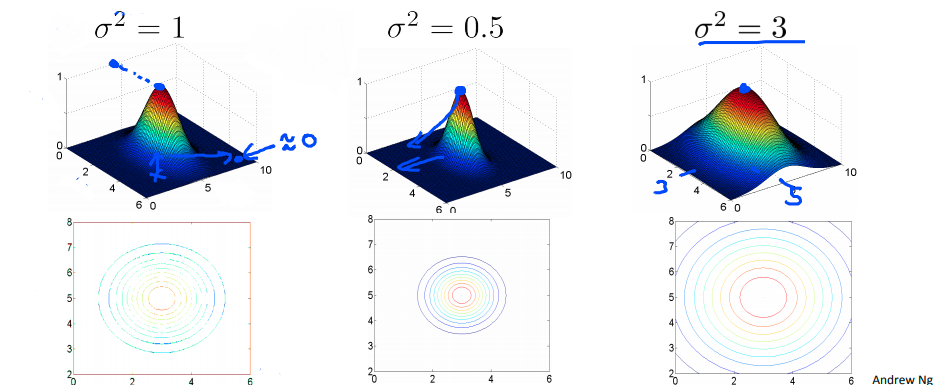
\includegraphics[width=0.8\textwidth]{svm-andrew.png}
	\caption{ Influențele aduse algoritmului de modificarea parametrului sigma în algoritmul de antrenare. }
	\label{fig:rev-proxy}
\end{figure}


Figura ~\ref{fig:rev-proxy} prezintă cum influențează clasificarea unui nou eveniment valoarea parametrului sigma din formula algoritmului de support vector machine.  Figura ~\ref{fig:rev-proxy} a fost preluata din slide-urile cursului de machine leraning susținut de Andrew Ng \cite{andrew_ng} \\


\section{SQL injection}

Atacurile de tipul SQL injection sunt realizate prin injectarea de cod executabil într-o bază de date. 

Procesul de interacționare cu o bază de date presupune realizarea de interogări asupra acesteia. În formularea acestor interogări, utilizatorul trebuie să prezinte interpretorului, sub formă de șiruri de caractere, numele tabelelor interogate sau valorile unor câmpuri specifice din acestea. Aceste șiruri de caractere sunt delimitate folosind caracterul "sau '. Atacurile de tipul SQL injection exploatează folosirea acestor delimitatori de șiruri de caractere, trimițând șiruri de caractere eronate intenționat către baza de date. Un utilizator rău intenționat poate să furnizeze astfel de șiruri de caractere către o baze de date prin intermediul oricărui procesator de conținut disponibil unui client al unei aplicații ce comunică cu o bază de date. Aceste șiruri de caractere delimitează prematur valoarea care este folosită în interogare, introducând după aceasta o serie de caractere pe care interpretorul le va trata că și cod executabil, oferindu-i astfel utilizatorului să execute operațiuni asupra bazei de date la care nu ar avea accesul în mod normal. Aceste operațiuni pot să reprezinte alterarea bazei de date sau obținerea de date confidențiale. \\



\begin{figure}[h]
	\centering
	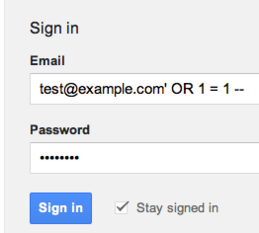
\includegraphics[width=0.4\textwidth]{259px-Sql_Injection_Login.png}
	\caption{Exemplu de atac realizat prin SQL injection.}
	\label{fig:sqli-example}
\end{figure}

Figura ~\ref{fig:sqli-example}  prezintă o tentativă de atac prin SQL injection în care în câmpul de validare a email-ului se încearcă injectarea de cod ce va fi executat în interogarea de validare a credentialelor. Prin prezența caracterului ' se escapează tot textul urmat după acesta ca fiind cod și nu un string ce face parte din câmpul de email. Operația logică "OR 1=1" va determina interpretorul să returneze adevărat(valid) pentru orice adresă de email introdusă înaintea caracterului  '. \\


\section{Adresele IP ale retelei Tor}
Rețeaua Tor reprezintă un softrware gratis de anonimizare a traficului pe internet. Numele este de fapt un acronim pentru "The Onion Router"(router-ul ceapă) care sugerează modul de funcționarea al acestuia, fiecare nod din rețea adăugând un strat extra de securitate celor precedente. Modul de funcționare al rețelei se bazează pe rutarea traficului prin cât mai multe noduri pentru a anonimiza și a face cât mai greu de urmărit traficul unei anumite persoane. Aceste noduri prin care traficul este direcționat sunt susținute gratis de către voluntari/utilizatori de Tor din întreaga lume. 

  
Pentru criptarea traficului rețeaua Tor folosește criptarea la nivelul aplicației în cea ce privește structura rețelelor de calculatoare(modelul OSI sau TCP/IP). Datele transmise sunt criptate, incluzând destinația, cu excepția nodului următor, astfel creându-se structura de "ceapă" asupra unui pachet. Selecția nodurilor prin care se face rutarea pachetelor este aleasă random. Fiecare pachet decriptează un "strat", aflând nodul următor pentru pachetul respectiv, nodul final decriptând datele inițiale și realizând transmisia către destinație, fără să îi comunice sursa pachetului. Întrucât în comunicarea pachetelor, pe parcursul rutelor parcurse, se cunoaște în permanență doar nodul următor, acest lucru împiedică monitorizarea traficului între sursă și destinație. 


Cu toate că rețeaua Tor oferă anonimitate de partea clientului, acest lucru nu se realizează și față de ea. Rețeaua nu se ascunde față de serviciile accesate prin intermediul ei. Astfel un site anume poate să detecteze dacă un anumit client îl accesează folosind rețeaua Tor sau nu. 

Întrucât rețeaua Tor nu își ascunde adresele IP folosite de către aceasta, identificarea lor și procurarea de date despre acestea este destul de ușoară. În proiectul propus s-a folosit un serviciu care furnizează gratuit astfel de date \cite{tot_status}(adresa IP, uptime etc.) și s-au folosit algoritmi proprii pentru procesarea acestor date, eliminând astfel necorectitudinea dintre utilizatorii rețelei. 

\begin{figure}[h]
	\centering
	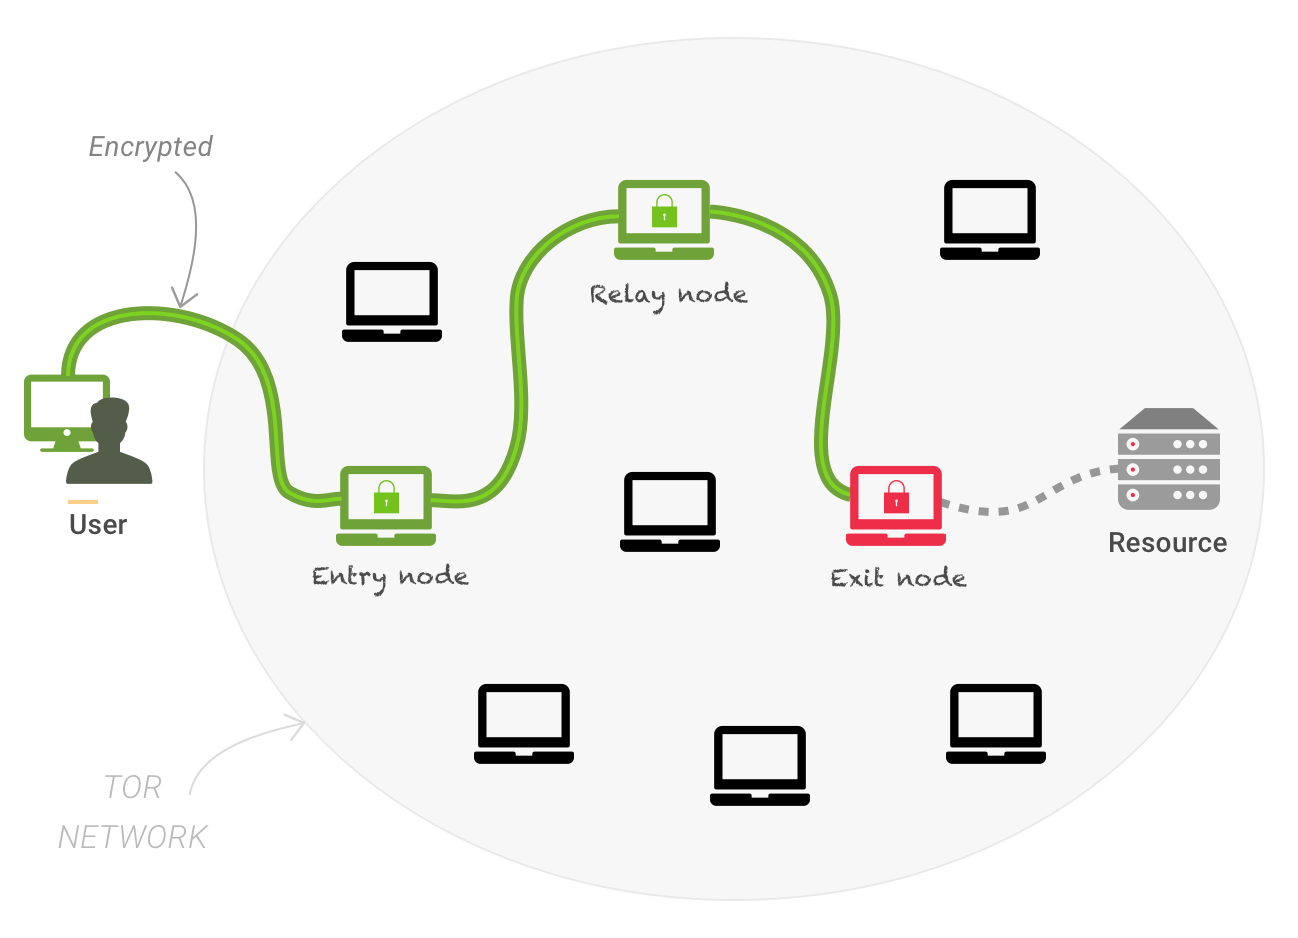
\includegraphics[width=0.6\textwidth]{can-you-hide-on-Tor-Network.png}
	\caption{ Exemplu de trafic realizat prin rețeaua Tor. }
	\label{fig:tor-example}
\end{figure}

Figura ~\ref{fig:tor-example}  prezintă principalele elemente folosite la rutarea traficului de la client la destinație prin intermediul rețelei Tor. \\


\section{Sistem de prevenire a intruziunilor}
Conform scurtei descrieri prezentate în capitolul anterior, un sistem de prevenire a intruziunilor are rolul de a filtra traficul dintre clienții unui server și serverul propriu-zis. 

Acest sistem funcționează liniar, adică este plasat direct între server și clienți acestuia. În cazul proiectului propus, componenta de bază pentru interceptarea traficului este realizată prin implementarea unui reverse proxy, oferind astfel caracteristica de interceptare și decriptare a traficului, ce permite analiza acestuia, dar și avantajele specifice utilizării unui reverse proxy. 

Pentru filtrarea traficului, un sistem de prevenire a intruziunilor implementează anumiți senzori care au rolul să inspecteze tot traficul ce trece prin sistem, realizând această inspecție în timp real. Datorită acestei verificări, orice pachet considerat malițios este oprit din a ajunge la serverul destinație. În proiectul propus, implementarea acestor senzori este realizată în două moduri. În cazul validării adreselor IP împotriva utilizatorilor de Tor se folosește o lista de IP-uri ce conține adrese frecvent utilizate de rețeaua Tor. În interiorul reverse proxy-ului, în momentul creării unei noi conexiuni, acesta verifică ca adresa IP ce solicită conectarea la server să nu fie conținută de lista menționată. În cazul detecției împotriva atacurilor de SQL injection, senzorul este implementat utilizând un model de support vector machine. În interiorul reverse proxy-ului în momentul interceptării unui request venit din exterior către rețeaua internă, acesta verifică dacă reqestul poate fi clasificat ca și tentativă de atac. În caz afirmativ blocând trecerea acestuia mai departe către server. 
\begin{figure}[h]
	\centering
	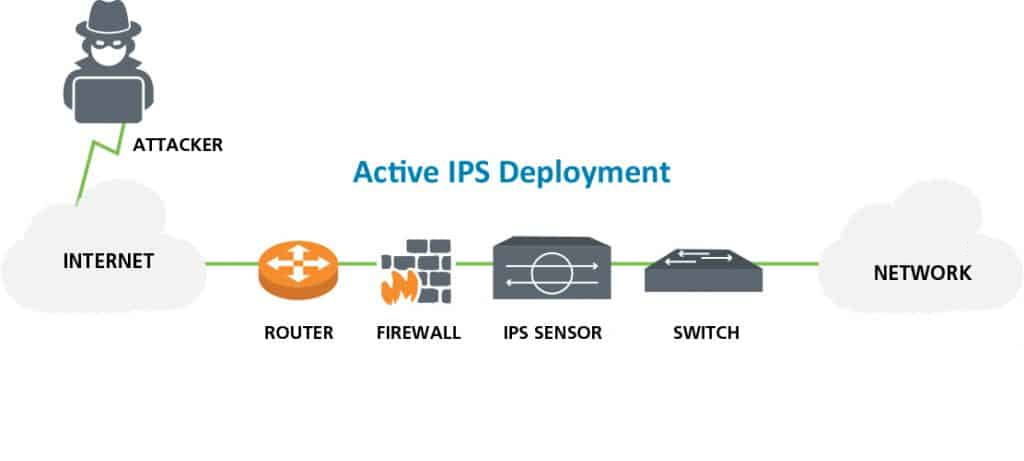
\includegraphics[width=0.6\textwidth]{IPS.png}
	\caption{ Integrarea unui sistem de prevenire a intruziunilor într-o rețea. }
	\label{fig:ips-2nd-example}
\end{figure}

Figura ~\ref{fig:ips-2nd-example} prezintă arhitectura unei rețele interne ce integrează un sistem de prevenire a intruziunilor pentru protejarea acesteia.  \\

Un sistem de prevenire a intruziunilor poate să efectueze oricare din următoarele acțiuni în momentul detectării unui eveniment malițios  \cite{ips_fire}:
\begin{itemize}
%	Terminates the TCP session that is being exploited by an outsider for the attack. It blocks the offending user account or source IP address that attempts to access the target host, application, or other resources unethically.
	\item  Să întrerupă sesiunea dintre client și server, în cazul în care clientul desfășoară sau încearcă să desfășoare activități malițioase în rețeaua protejată de sistem. Acest lucru se poate realiza prin blocarea anumitor credentiale asociate cu utilizatorul respectiv sau prin blocarea adresei IP a acestuia. 
	\item  În condițiile în care un sistem de prevenire a intruziunilor detectează/clasifica o activitate ca fiind malițioasă, acesta poate să ia măsuri automat pentru a preveni un astfel de atac pe viitor(ex: în momentul detectării unei tentative de atac prin SQL injection, sistemul de prevenire a intruziunilor poate să blocheze în mod automat adresa IP a utilizatorului ce încearcă să facă atacul, nepermițându-i acestuia să se mai conecteze la serverul destinație pentru un anumit interval de timp sau până la intervenția unui administrator). 
	\item  O alata abordare posibilă în momentul declanșării unui eveniment malițios este alterarea traficului astfel încât să elimine conținutul malițios din acesta. Pentru realizarea acestui lucru, un sistem de prevenire a intruziunilor poate să șteargă atașamente infectate din interiorul unui mail, să altereze conținutul unui pachet sau să omită transmiterea mai departe a unor pachete. 
	
\end{itemize}

